%!TEX root = ../thesis.tex

\chapter{Discussion}
\label{ch:discussion}
The implementation of digital asset management through issuance of \ac{NFT}s represents a milestone in the generation of decentralized secure frameworks for industrial applications.

The implicit security of Blockchain with Hyperledger management and the privacy such technology offers will allow different organizations to participate and cooperate securely, but not anonymously. 

All parties will be able to acknowledge data ownership. If desired, data could be encrypted as well and managed trough additional smart contracts. In addition to this, \ac{IPFS} network is able to control, distribute and manage the added data as a \ac{DFS}. The final simulation of the environment allows testers, to acknowledge the workflow of the framework and further expand its capabilities in a modular way.

\section{Results}
The simulation was performed with the following operations:

\begin{enumerate}
    \item Minting NFT with Text data ~ 10KB
    \item Minting NFT with Image data ~ 200KB
    \item Minting NFT with Bin data ~ 100MB
    \item Minting NFT with a file of ~850MB
\end{enumerate}

The highest resource consuming process for the system is whenever data with high space resources is about to be minted. The communication with the server and IPFS network create a bottle neck in the simulation process and by running the resources locally.

\begin{table}[h!]
\begin{center}
\begin{tabular}{ |c|c|c|c|  }
 \hline
 \multicolumn{4}{|c|}{NFT Statistics} \\
 \hline
 No & File type & Size  & Elapsed time (s)\\
 \hline
 1   & Text     & 10KB &   0.5  \\
 2   & Image    & 200KB &   1.3 \\
 3   & PDF      & 100MB &   8.3 \\
 4   & Bin      & 850MB &   $\infty$ \\
 
 \hline
\end{tabular}
\caption{NFT Statistics.}
\label{table:NFTStats}
\end{center}
\end{table}

Whenever trying to mint an NFT File larger than 500 MB (previous tests were made with other files) the blockchain system, or at least the \ac{API} server takes significantly larger amount time than expected to submit the data. Although this might be a parameter or server side configuration, it certainly refrains users from submitting large amounts of information.

Final results of the built application indicate that it is potentially feasible to create decentralized systems specialized in data management and control for industrial purposes while dealing with chunks of data. For text data it is relatively easy to mint, submit and visualize under the IPFS Server.

\subsection{Infrastructure statistics}
The following statistics were performed by running \textit{docker stats} command where they where later on plotted.
\begin{figure}[h!]
        \centering
        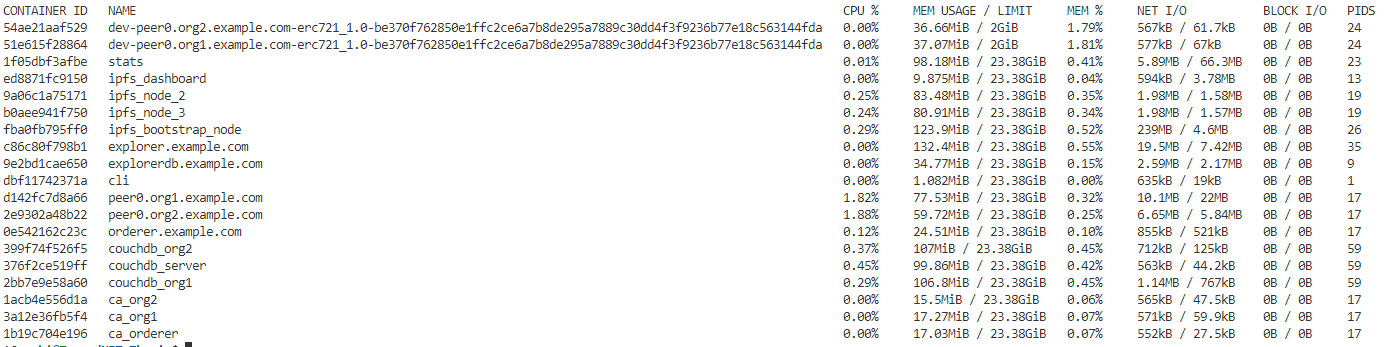
\includegraphics[width=15cm]{img/Docker_Stats.png}
        \caption{Docker statistics from current containers}
        \label{fig:dockerStats}
\end{figure}

\subsubsection{Memory Usage}
The image \ref{fig:dockerMem} shows the amount of memory used by all the servers. The containers with higher numbers are the ones used to provide statistics and insights. in Orange: The container to run statistics, whereas in blue the container running Hyperledger explorer \ac{UI}. The unit of measure has been performed in \ac{MiB}.
\begin{figure}[h!]
        \centering
        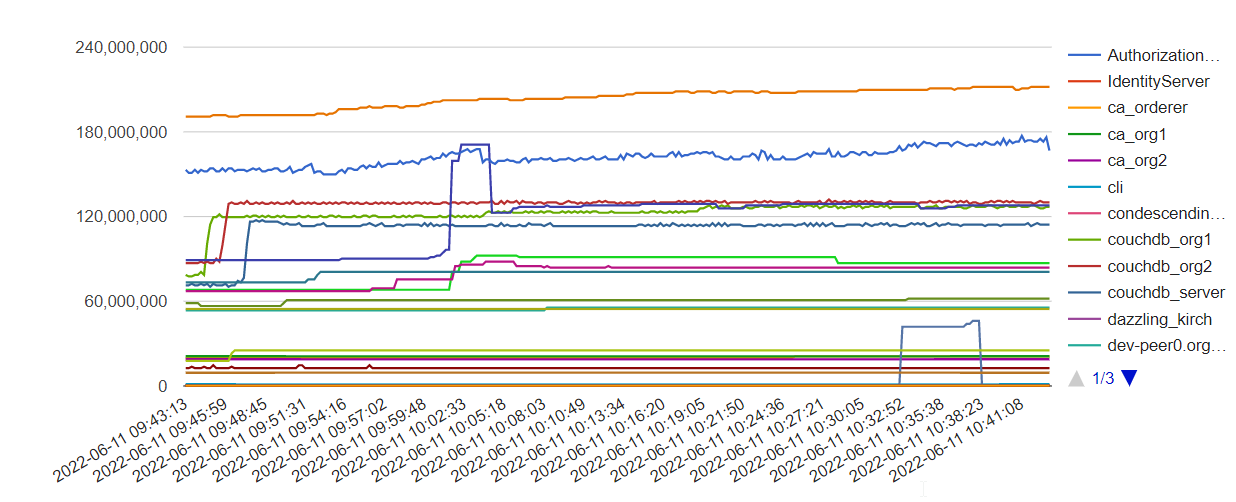
\includegraphics[width=15cm]{img/Docker_Mem.png}
        \caption{Infrastructure Memory Usage. Unit of measure in MiB}
        \label{fig:dockerMem}
\end{figure}

\subsubsection{CPU Usage}
Image \ref{fig:dockerCPU} shows the amount of \ac{CPU} in terms of \ac{IPS} executed. The peaks shown correspond to the IPFS network.
\begin{figure}[h!]
        \centering
        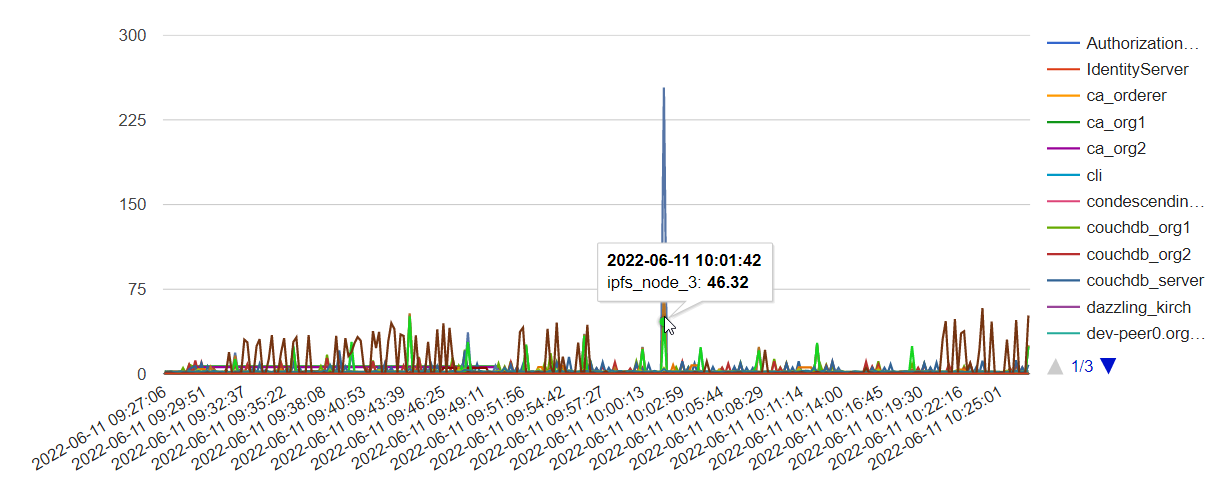
\includegraphics[width=15cm]{img/Docker_CPU.png}
        \caption{Infrastructure CPU Usage in IPS}
        \label{fig:dockerCPU}
\end{figure}

\subsubsection{Network inputs}
Image \ref{fig:dockerNetIn} shows all  network inputs consumed by each container. In color blue it can be highlighted that IPFS network is the node taking most of the network inputs due to the amount of memory consumed after minting large file sizes for the \ac{NFT}. Unit of measure is in \ac{kB}
\begin{figure}[h!]
        \centering
        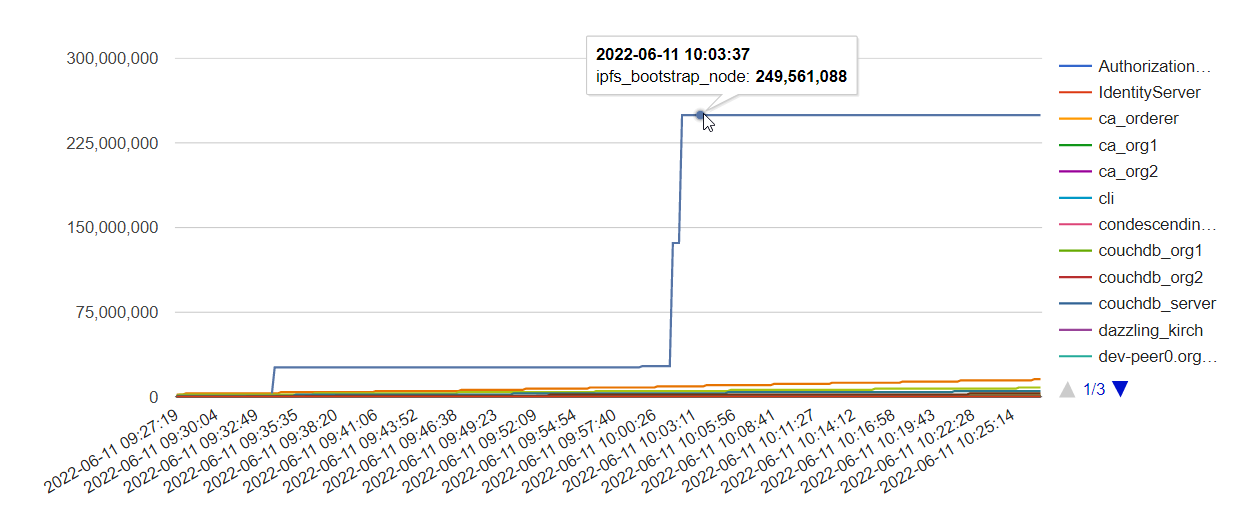
\includegraphics[width=15cm]{img/Docker_NetIn.png}
        \caption{Network Inputs}
        \label{fig:dockerNetIn}
\end{figure}

\subsubsection{Network outputs}
Image \ref{fig:dockerNetOut} shows all network outputs sent by each container. At the top the container used to run the statistics has the most of data sent. In In second place the peer node corresponding to organization one presents the one with the most information transmitted. Unit of measure is in \ac{kB}.
\begin{figure}[h!]
        \centering
        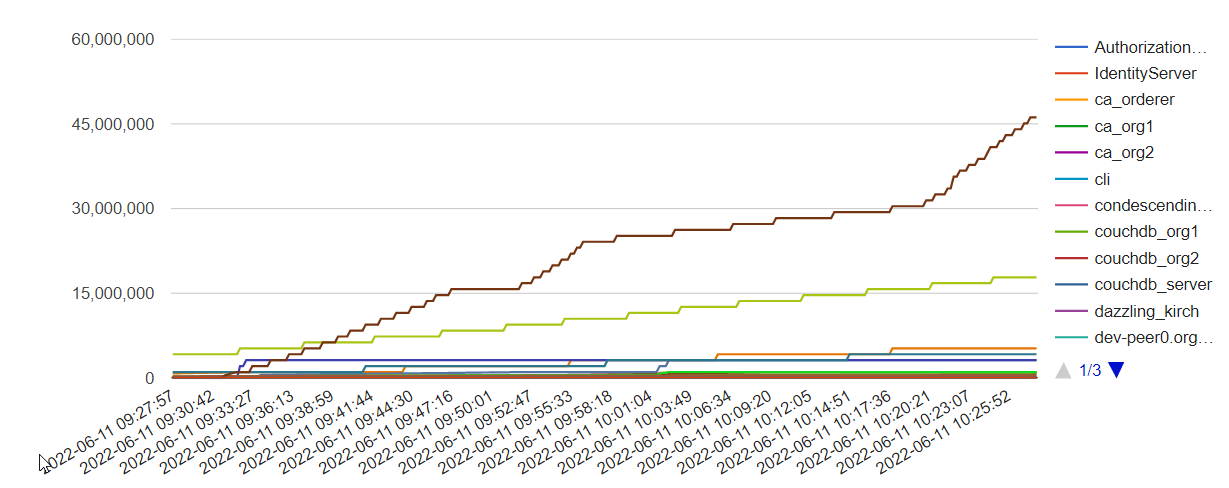
\includegraphics[width=15cm]{img/Docker_NetOut.png}
        \caption{Network Outputs}
        \label{fig:dockerNetOut}
\end{figure}



\subsection{Benchmarking and Blockchain metrics evaluation}
Hyperledger framework has a benchmark tool used to measure the performance and behavior of the blockchain, test it and evaluate it under stress scenarios to check its latency and behaviour under heavy usage. Tables \ref{table:Benchmark1} and \ref{table:Benchmark2} show the results thrown in raw data. Figure \ref{fig:CaliperBenchmark} presents relevant information about the usage and network stress results. as an HTML report, which is also available at:
\url{https://htmlpreview.github.io/?https://raw.githubusercontent.com/asahicantu/NFT-Thesis/main/caliper-benchmarks/report.html} Units of measure for the data are in \ac{s} and \ac{TPS}.

\begin{table}[h!]
\begin{center}
\begin{tabular}{ |c|c|c|c|c|c|  }
 \hline
 \multicolumn{6}{|c|}{Blockchain benchmark Part I.} \\
 \hline
 Name & Succ  & Fail  & Send Rate (TPS) & Max Latency(s) & Min Latency (s)\\
 \hline
 MintNFT.           & 5000   & 0 &   15.0  &  2.19 & 0.10  \\
 Query all NFTS.    & 9819   & 0 &   338.2 &  0.06 & 0.01   \\
 \hline
\end{tabular}
\caption{Blockchain Benchmark using Hyperledger Caliper Part I.}
\label{table:Benchmark1}
\end{center}
\end{table}

\begin{table}[h!]
\begin{center}
\begin{tabular}{ |c|c|c|  }
 \hline
 \multicolumn{3}{|c|}{Blockchain benchmark} \\
 \hline
 Name & Avg Latency (s) & Throughput (TPS)\\
 \hline
 MintNFT.           & 0.43 & 14.9 \\
 Query all NFTS.    & 0.02 & 338.1 \\
 \hline
\end{tabular}
\caption{Blockchain Benchmark using Hyperledger Caliper.}
\label{table:Benchmark2}
\end{center}
\end{table}

 \begin{figure}[!h]
        \centering
        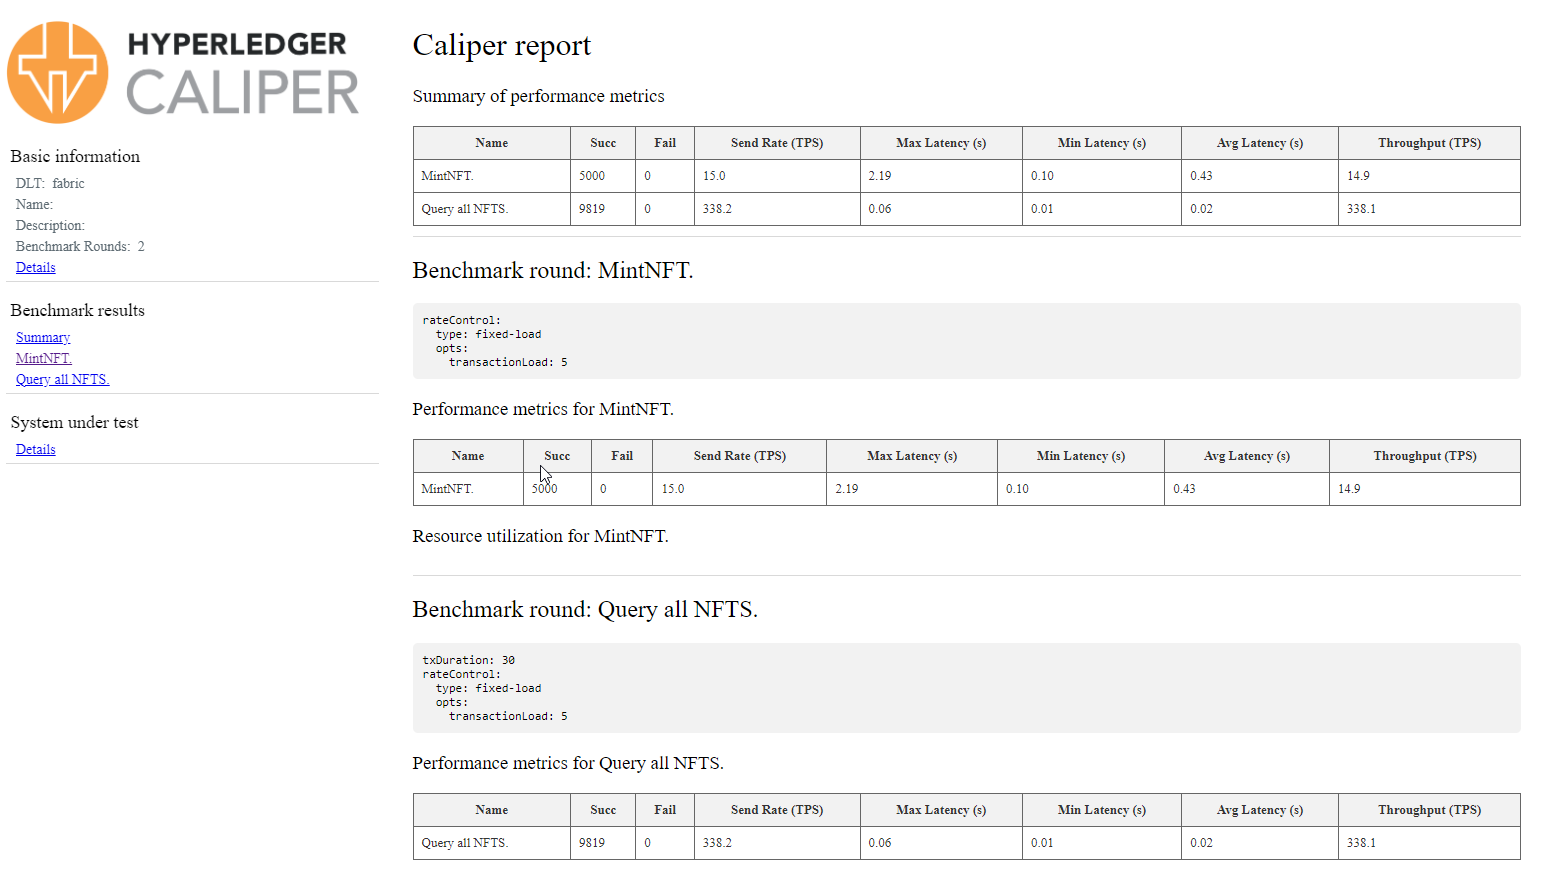
\includegraphics[width=15cm]{img/Caliper.png}
        \caption{Hyperledger Caliper Benchmark results.}
        \label{fig:CaliperBenchmark}
    \end{figure}
